\chapter{Конструкторская часть}
В данном разделе будут представлены схемы алгоритмов сортировки (гномья сортировка, поразрядная сортировка, сортировка выбором) и вычисления трудоемкости данных алгоритмов.
 

\section{Алгоритм гномьей сортировки}

На рисунке \ref{img:gnome_sort.png} приведена схема алгоритма гномьей сортировки.
\\
\\
\\
\\
\\
\\
\\
\\
\\
\\
\\
\\
\\
\\
\\
\\
\\
\\
\\
\\
\\
\\

\img{230mm}{gnome_sort.png}{Схема алгоритма гномьей сортировки}


\FloatBarrier
\section{Алгоритм поразрядной сортировки}
На рисунках \ref{img:radix_sort1.png} и \ref{fig:radix_sort2} приведена схема алгоритма поразрядной сортировки.
\\
\\
\\
\\
\\
\\
\\
\\
\\
\\
\\
\\
\\
\\
\\
\\
\\
\\
\\
\\
\\
\\
\\
\\
\\
\\
\\
\\

\img{230mm}{radix_sort1.png}{Схема алгоритма поразрядной сортировки}


\begin{figure}[H!]
	
	\centering{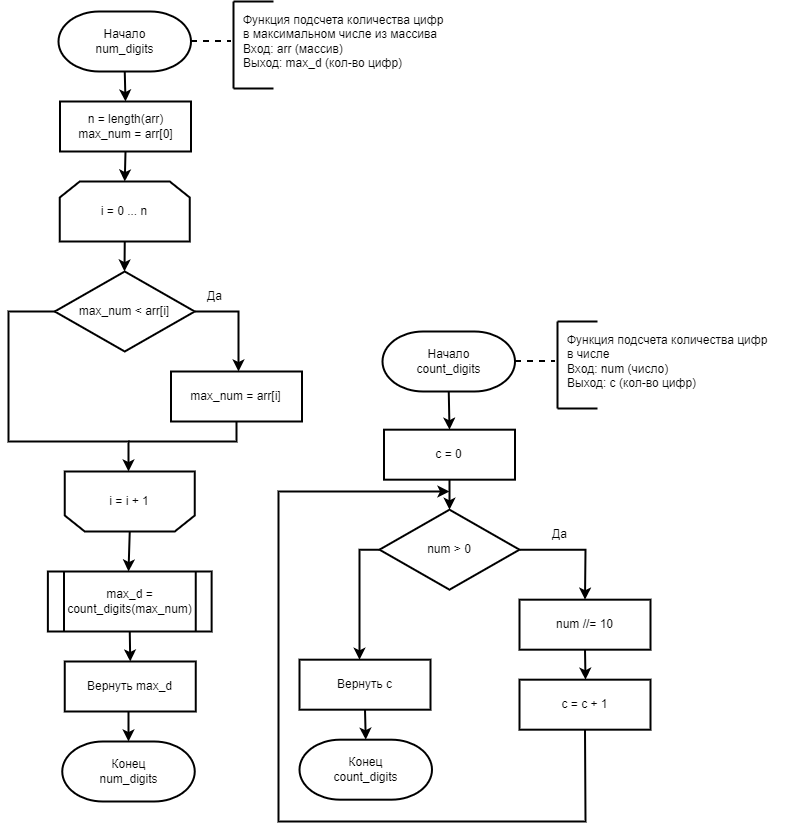
\includegraphics[scale=0.65]{inc/radix_sort2.png}}
		
		\caption{Схема алгоритма поразрядной сортировки}
		
		\label{fig:radix_sort2}
		
	\end{figure}

\FloatBarrier
\section{Алгоритм сортировки выбором}
На рисунке \ref{img:selection_sort.png} приведена схема алгоритма сортировки выбором.
\\
\\
\\
\\
\\
\\
\\
\\
\\
\\
\\
\\
\\
\\
\\
\\
\\
\\
\\
\\
\\
\\
\\
\\
\\
\\
\\
\\

\img{230mm}{selection_sort.png}{Схема алгоритма сортировки выбором}



\FloatBarrier
\section{Оценка трудоемкости алгоритмов сортировки}

Для последующего вычисления трудоемкости необходимо ввести следующую модель вычислений:
\begin{itemize}
	\item базовые операции с трудоемкостью 2: /, /=, *, *=, \%, \%=;
	\item базовые операции с трудоемкостью 1: +, ++, +=, -, --, -=, ==, !=, <, >, <=, >=, <<, >>, [];
	\item трудоемкость цикла: Fцикла = Fиниц. + Fсравн. + M * (Fтела + Fинк. + Fсравн.), где Fиниц., Fсравн., Fтела, Fинк. - трудоемкости инициализации,  проверки условия цикла, тела цикла и инкрементирования соответственно, а M - количество итераций;
	\item трудоемкость условного оператроа: F$_{if}$ = Fсравн. + 
	\begin{equation}
		+
		\left[ 
		\begin{array}{c} 
			min(f1, f2) - $лучший случай$\\
			max(f1, f2) - $худший случай$\\
		\end{array}
		\right.,\\
	\end{equation}где Fсравн., f1, f2 - трудоемкости проверки условия, первого блока и второго блока, соответственно.
	
\end{itemize}

Обозначим во всех последующих вычислениях размер массивов как N, K - количество допорлнительных итераций из-за обменов элементов.

\subsection{Алгоритм гномьей сортировки}

Трудоемкость алгоритма сортировки выбором состоит из:
\begin{itemize}
	\item Трудоемкость цикла $while(i < N)$, которая равна (\ref{while:gnome}):
	\begin{equation}
		\label{while:gnome}
		f_{while} = 2 + 2 \cdot (N - 1) \cdot f_{if} \cdot (K + 1)
	\end{equation}
	\item Трудоемкость условия в цикле, которая равна (\ref{while:gnome_if}):
	\begin{equation}
		\label{while:gnome_if}
		f_{if} = 4 + \begin{cases}
			0, & \text{л.с.}\\
			9, & \text{х.с.}\\
		\end{cases}
	\end{equation}
	\item Количество дополнительных итераций из-за обменов элементов (\ref{while:gnome_k}):
	\begin{equation}
		\label{while:gnome_k}
		K = \begin{cases}
			0, & \text{л.с.}\\
			N - 1, & \text{х.с.}\\
		\end{cases}
	\end{equation}
\end{itemize}

Трудоемкость в лучшем случае (\ref{while:gnome_best}):
\begin{equation}
	\label{while:gnome_best}
	f_{best} = 8N - 6 \approx 8N = O(N)
\end{equation}

Трудоемкость в худшем случае (\ref{while:gnome_worst}):
\begin{equation}
	\label{while:gnome_worst}
	f_{worst} = 26N^2 - 13N + 2 \approx 26N^2 = O(N^2)
\end{equation}


\subsection{Алгоритм поразрядной сортировки}

Трудоемкость алгоритма сортировки выбором состоит из:
\begin{itemize}
    \item Трудоемкость подсчета m для цикла функции radix\_sort, где m - количество цифр в максимальном числе из массива (\ref{for:radix_m_count}):
    \begin{equation}
		\label{for:radix_m_count}
		f_{count\_m} = 1 + f_{num\_digits}
	\end{equation}
	\item Трудоемкость функции num\_digits (\ref{func:num_dig}):
	\begin{equation}
		\label{func:num_dig}
		f_{num\_digits} = 4 + f_{for} + f_{count\_digits}
	\end{equation}
	\item Трудоемкость сравнения, инкремента цикла функции num\_digits, а также зависимых только от него операций, по $d \in [0...N)$, которая равна (\ref{for:num_dig}):
	\begin{equation}
		\label{for:num_dig}
		f_{for} = N * (2 + f_{if})
	\end{equation}
	\item Трудоемкость условия в цикле, которая равна (\ref{for:radix_if}):
	\begin{equation}
		\label{for:radix_if}
		f_{if} = 2 + \begin{cases}
			0, & \text{л.с.}\\
			2, & \text{х.с.}\\
		\end{cases}
	\end{equation}
	\item Трудоемкость функции count\_digits (\ref{func:count_dig}):
	\begin{equation}
		\label{func:count_dig}
		f_{count\_digits} = 1 + f_{while}
	\end{equation}
	\item Трудоемкость цикла $while(num > 0)$, где m - количество цифр в максимальном числе из массива, равна(\ref{while:count_dig}):
	\begin{equation}
		\label{while:count_dig}
		f_{while} = m * (2 + 2) = 4m
	\end{equation}
	\item Трудоемкость сравнения, инкремента внешнего цикла функции radix\_sort, а также зависимых только от него операций, по $d \in [0...m)$, где m - количество цифр в максимальном числе из массива, которая равна (\ref{for:radix_outer}):
	\begin{equation}
		\label{for:radix_outer}
		f_{outer} = 1 + m \cdot (42 + 11) + f_{inner} = 1 + 53m + f_{inner}
	\end{equation}
	\item Суммарная трудоемкость внутренних циклов функции radix\_sort по $i \in [0...N)$, которая равна (\ref{for:radix_inner}):
	\begin{equation}
		\label{for:radix_inner}
		f_{inner} = m + N \cdot (2 + 3 + 6 + 2 \cdot \frac{(m - 1) \cdot m}{2}) = m + N \cdot (11 + m^2 - m)
	\end{equation}
\end{itemize}

Трудоемкость в лучшем случае, где m - количество цифр в максимальном числе из массива (m << N), равна (\ref{for:radix_best}):
\begin{equation}
	\label{for:radix_best}
	f_{best} = N \cdot(m^2 - m) + 58m + 15N + 7\approx N*(m^2 - m + 15) = O(N)
\end{equation}

Трудоемкость в худшем случае, где m - количество цифр в максимальном числе из массива (m << N), равна (\ref{for:radix_worst}):
\begin{equation}
	\label{for:radix_worst}
	f_{worst} = N \cdot(m^2 - m) + 58m + 17N + 7\approx N*(m^2 - m + 17) = O(N)
\end{equation}

\subsection{Алгоритм сортировки выбором}

Трудоемкость алгоритма сортировки выбором состоит из:
\begin{itemize}
	\item Трудоемкость сравнения, декремента внешнего цикла, а также зависимых только от него операций, по $i \in [N-1...0)$, которая равна (\ref{for:selection_outer}):
	\begin{equation}
		\label{for:selection_outer}
		f_{outer} = 3 + (5 + f_{ifout}) \cdot (N - 1)
	\end{equation}
	\item Трудоемкость условия во внешнем цикле, которая равна (\ref{for:selection_if_outer}):
	\begin{equation}
		\label{for:selection_if_outer}
		f_{ifout} = 1 + \begin{cases}
			0, & \text{л.с.}\\
			7, & \text{х.с.}\\
		\end{cases}
	\end{equation}
	\item Суммарная трудоемкость внутренних циклов, количество итераций которых меняется в промежутке $[N-2..0]$, которая равна (\ref{for:selection_inner}):
	\begin{equation}
		\label{for:selection_inner}
		f_{inner} = 2 \cdot (N - 1) + f_{ifin} \cdot \frac{(N - 2) \cdot (N - 1)}{2}
	\end{equation}
	\item Трудоемкость условия во внутреннем цикле, которая равна (\ref{for:selection_if_inner}):
	\begin{equation}
		\label{for:selection_if_inner}
		f_{ifin} = 3 + \begin{cases}
			0, & \text{л.с.}\\
			1, & \text{х.с.}\\
		\end{cases}
	\end{equation}
\end{itemize}

Трудоемкость в лучшем случае (\ref{for:selection_best}):
\begin{equation}
	\label{for:selection_best}
	f_{best} = \frac{3}{2}N^2 + \frac{9}{2}N - 2\approx \frac{3}{2}N^2 = O(N^2)
\end{equation}

Трудоемкость в худшем случае (\ref{for:selection_worst}):
\begin{equation}
	\label{for:selection_worst}
	f_{worst} = 2N^2 + 9N - 8 \approx 3N^2 = O(N^2)
\end{equation}


\section*{Вывод}

В данном разделе были разработаны схемы алгоритмов сортировки (гномья сортировка, поразрядная сортировка, сортировка выбором). Для каждого из них были рассчитаны и оценены лучшие и худшие случаи.
